\documentclass[11pt]{article}
\usepackage[margin=1in]{geometry}
\usepackage{lmodern}
\usepackage[T1]{fontenc}
\usepackage{amsmath,amssymb}
\usepackage{booktabs}
\usepackage{tabularx}
\usepackage{graphicx}
\usepackage{float}
\usepackage{xcolor}
\usepackage{hyperref}
\usepackage{natbib}
\usepackage{enumitem}
\hypersetup{colorlinks, linkcolor=blue!50!black, citecolor=blue!50!black, urlcolor=blue!50!black}
\setlist{itemsep=2pt, topsep=4pt}
\newcommand{\takeaway}[1]{\noindent\textbf{#1}\par\smallskip}

\title{When Trading Dries Up:\\A Liquidity Signal for a Long-Only Fund}
\author{Silver Fund Research}
\date{November 2026}

\begin{document}
\maketitle

\begin{abstract}
\noindent
When trading in a stock suddenly dries up, the stock keeps falling for months: about 3\% behind similar
stocks over the next year, beyond anything the fund's existing scores capture. We turn this into a Grinold--Kahn
alpha and trade it with the fund's optimizer. Rebalanced daily, the long-only portfolio earns $+0.19\%$ a year in
2011--2018 and $+0.51\%$ a year (information ratio 1.05) in 2019--2024, years we held back and ran only once.
The effect is real but small, so it belongs as one input to the fund's alpha.
\end{abstract}

% ======================================================================
\section{The idea}
\takeaway{Most investors avoid illiquid stocks. When a stock's trading collapses, it has to pass to a small group of patient
buyers, and that slow hand-off pushes its price down for months.}

\paragraph{Two kinds of investors.} Most investors, such as mutual funds that face daily redemptions, institutions that
size positions by trading volume, and active traders, want stocks they can buy and sell quickly and cheaply. A much smaller
group with long horizons is willing to hold illiquid stocks, but only at a lower price, which earns them a slightly higher
expected return \citep{amihud1986}. Stocks therefore sort into clienteles: liquid stocks are held by the many, illiquid
stocks by the patient few.

\paragraph{A collapse forces a hand-off.} When trading in a stock suddenly collapses, the stock no longer suits the investors
who own it. They want out, and the stock has to pass to the patient group. Two frictions make this slow. Sellers can exit only
a little at a time, because volume has dried up and selling faster would push the price down sharply. And the patient group
is small, with limited capital, so each sale needs a slightly lower price to find a buyer. The price walks down step by step
until the stock is held by investors who are content at the new, lower price.

\paragraph{Why the drift is not traded away.} An investor who saw the decline coming would sell the stock short, but shorting
small, illiquid stocks is expensive and often impossible to arrange. So the decline is predictable and persists, as
\citet{bali2014} also find.

\paragraph{What this predicts.} The story is about a \emph{change} in liquidity, not its level. It makes five predictions,
each checked in Section~\ref{sec:evidence}:
\begin{enumerate}
  \item After a collapse, the stock earns lower returns than similar stocks whose liquidity did not collapse.
  \item The decline is gradual and strongest at first, while most holders are trying to leave.
  \item It is strongest in small stocks, where the pool of patient buyers is smallest.
  \item It is driven by the fall in trading volume, the friction that slows the exit, rather than by large price moves.
  \item Stocks that are \emph{already} illiquid, and already held by patient investors, earn slightly \emph{more}: the
        patient group's reward for holding them.
\end{enumerate}

\paragraph{The question for the fund.} The Silver Fund is long-only and already trades six scores: idiosyncratic
volatility, momentum, reversal, Barra momentum, beta and Barra reversal. A new signal is worth adding only if it carries
information those scores do not, and if the fund can profit from it while only ever holding \emph{less} of a stock than
the benchmark, never shorting it.

% ======================================================================
\section{Does the evidence fit?}\label{sec:evidence}
\takeaway{All five predictions hold: flagged stocks fall about 3\% behind similar stocks over a year.}

We flag a stock when its trading collapses relative to its own past year (Section~\ref{sec:signal}) and compare it with
\emph{similar stocks}: those of the same size and the same prior illiquidity on the same day. Comparing with similar stocks
separates the collapse itself from simply being a small or illiquid stock. Returns throughout are \emph{abnormal returns}:
the part of each stock's return not explained by the market and the usual industry and style factors (Barra's specific return).

\begin{table}[H]
\centering
\caption{The five predictions against the data, 2006--2018.}\label{tab:evidence}
\small
\begin{tabularx}{\textwidth}{p{0.36\textwidth}X}
\toprule
Prediction & Evidence \\
\midrule
1.\ Lower returns afterwards & $-2.9\%$ against similar stocks after a year ($t=-3.6$). In monthly regressions with size,
  prior illiquidity, momentum and reversal as controls, flagged stocks earn 0.18\% a month less ($t=2.5$; Appendix). \\
2.\ Gradual, strongest at first & $-0.5\%$ after one month, $-0.9\%$ after three, $-1.7\%$ after six, $-2.9\%$ after twelve. \\
3.\ Strongest in small stocks & $-2.9$ to $-3.4\%$ after a year in the smaller size groups; $-0.8\%$ ($t=-1.4$) in the largest fifth. \\
4.\ Driven by the fall in trading & Measured on the volume part alone, the worst tenth lags by 0.58\% a month ($t=-6.5$);
  on the price-move part alone, by 0.24\% ($t=-3.8$). \\
5.\ Already-illiquid stocks earn slightly more & Holding size fixed, the most illiquid stocks earn about 0.8\% a month more
  than the most liquid ($t=2.8$). \\
\bottomrule
\end{tabularx}
\end{table}

\begin{figure}[H]
\centering
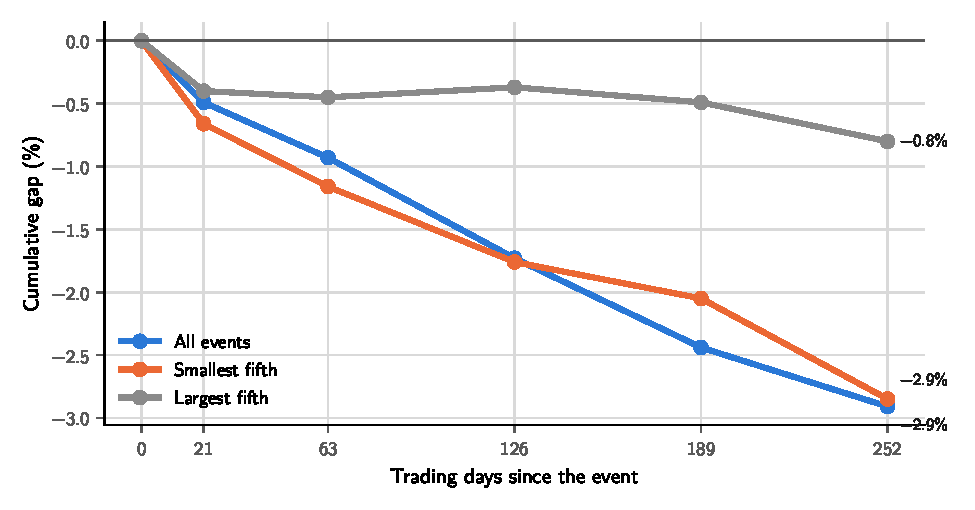
\includegraphics[width=0.58\linewidth]{figures/matched_drift.pdf}
\caption{Abnormal return after a liquidity collapse minus similar stocks, events 2006--2018.}\label{fig:drift}
\end{figure}

The effect is also new to the fund: removing the fund's six scores from the signal first leaves it intact (its
information coefficient rises from 0.005 to 0.015, $t=6.0$). One practical catch follows from prediction 3. The effect
lives in small stocks, which hold little weight in the benchmark, and a long-only fund can underweight a stock only down to zero.

% ======================================================================
\section{The pipeline}\label{sec:signal}
\takeaway{Seven steps, from raw data to a backtest tested once on held-back years.}

\begin{enumerate}
  \item \textbf{Data:} Barra US daily data through \texttt{sf\_quant}: returns, prices, volume, risk model, benchmark
        weights and bid--ask spreads. Benchmark stocks priced above \$5.
  \item \textbf{Liquidity shock:} the price move per dollar traded (Amihud illiquidity, \citealp{amihud2002}) over the last month, compared
        with the stock's own average over the previous year.
  \item \textbf{Remove what the fund knows:} each day, regress the shock across stocks on the fund's six scores and keep
        the standardized residual, $Z$.
  \item \textbf{Events:} a stock has an event when its $Z$ enters the worst 5\% after 21 quiet days.
  \item \textbf{Alpha:} the Grinold--Kahn form, expected abnormal return $=$ forecasting skill $\times$ the stock's
        volatility $\times$ the signal, estimated from past years only.
  \item \textbf{Optimizer:} choose active weights to maximize expected active return minus a penalty for active risk,
        with zero beta to the benchmark and 5\% tracking error, with and without the long-only rule.
  \item \textbf{Test:} backtest 2011--2018, freeze the design, then run 2019--2024 once.
\end{enumerate}

% ======================================================================
\section{Building the signal}
\takeaway{Each choice either isolates the collapse or matches how slowly its effect plays out.}

\begin{table}[H]
\centering
\caption{Design choices and why we made them.}\label{tab:choices}
\small
\begin{tabularx}{\textwidth}{p{0.40\textwidth}X}
\toprule
Choice & Why \\
\midrule
Compare each stock's liquidity with \emph{its own} past year &
  We want a \emph{collapse} in trading, not a stock that is always illiquid. \\
Remove the fund's six scores before anything else &
  The signal should only get credit for information the fund does not already have. \\
An event is entering the worst 5\% after 21 quiet days; positions are held for weeks, not days &
  The drift lasts months. A daily score turns over too fast to hold a position while the drift arrives. \\
Estimate everything against similar stocks (same size, same prior illiquidity) &
  Isolates the collapse from simply being small or illiquid. \\
Alpha $=$ stock's volatility $\times$ expected drift per unit of risk, by time since the event (1--21 and 22--63 days) &
  This is Grinold--Kahn with an on/off signal. Without the volatility term the model overrated calm stocks (Figure~\ref{fig:vol}). \\
Re-estimate every January from earlier years only; never allow a positive alpha &
  No look-ahead. The story predicts only underperformance, so a positive estimate is noise. \\
Optimizer: zero beta, 5\% tracking error, net-zero active weight among similar stocks &
  The portfolio bets on the collapse, not on the market, size or illiquidity. \\
Rebalance daily; charge no trading costs, but report them &
  Most of the drift comes in the first weeks. The signal is one input to the fund's alpha, where trades net out. \\
\bottomrule
\end{tabularx}
\end{table}

\paragraph{Why volatility belongs in the alpha.} In the Grinold--Kahn form, a forecast scales with the stock's volatility:
the same signal is worth more in a volatile stock than in a calm one. An earlier version left that term out and gave every
flagged stock the same alpha. The optimizer then favored calm stocks, where the same expected drift looks like a better deal
at lower risk. But calm stocks delivered about a third of the predicted return, and volatile ones half again as much
(Figure~\ref{fig:vol}). The drift does scale with volatility, so the final alpha does too.

\begin{figure}[H]
\centering
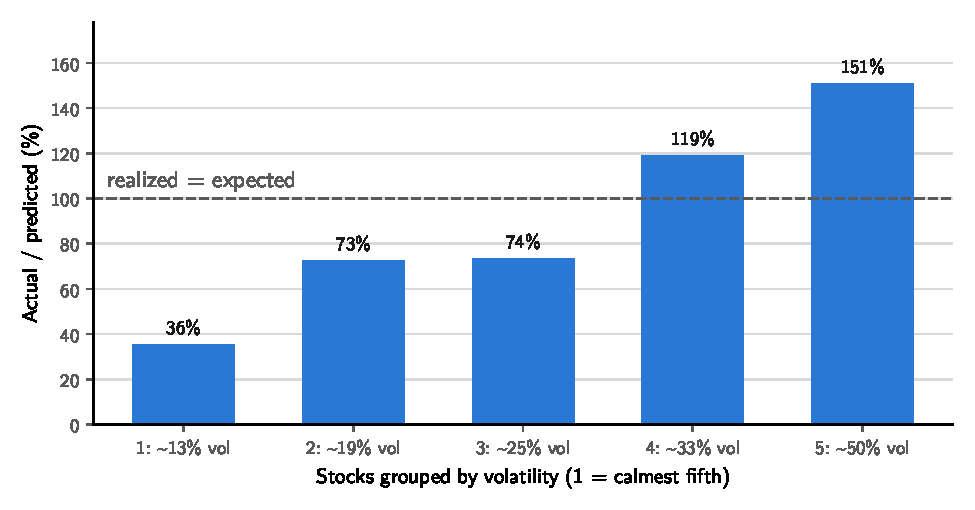
\includegraphics[width=0.72\linewidth]{figures/vol_check.pdf}
\caption{Earlier version without volatility in the alpha: actual return as \% of predicted, by volatility fifth (2011--2018).}\label{fig:vol}
\end{figure}

% ======================================================================
\section{Results}
\takeaway{Traded daily, the signal works long-only and held up in the held-back years; traded monthly, it does not.}

We run two portfolios. \emph{No limits} shows the signal's full strength. \emph{No shorting} adds the fund's long-only
rule: a stock's weight can be cut to zero but not below. The fundamental law says the information ratio grows with
forecasting skill and the number of independent bets, $IR = IC\sqrt{BR}$; a constraint keeps only part of that, and the
transfer coefficient (TC) measures how much: $IR = TC \times IC\sqrt{BR}$ \citep{clarke2002}.

\begin{table}[H]
\centering
\caption{Active return per year, information ratio and transfer coefficient. No trading costs charged.}\label{tab:results}
\small
\begin{tabular}{lrrrrrr}
\toprule
 & \multicolumn{3}{c}{2011--2018} & \multicolumn{3}{c}{2019--2024 (held back)} \\
\cmidrule(lr){2-4}\cmidrule(lr){5-7}
Portfolio & Return & IR & TC & Return & IR & TC \\
\midrule
Daily, no limits & +6.84\% & 1.17 & --- & +7.43\% & 1.21 & --- \\
Daily, no shorting & +0.19\% & 1.82 & 0.44 & +0.51\% & 1.05 & 0.36 \\
Monthly, no limits & +2.92\% & 0.48 & --- & +3.58\% & 0.54 & --- \\
Monthly, no shorting & +0.08\% & 0.82 & 0.44 & $-$0.02\% & $-$0.05 & 0.36 \\
\bottomrule
\end{tabular}
\end{table}

\begin{figure}[H]
\centering
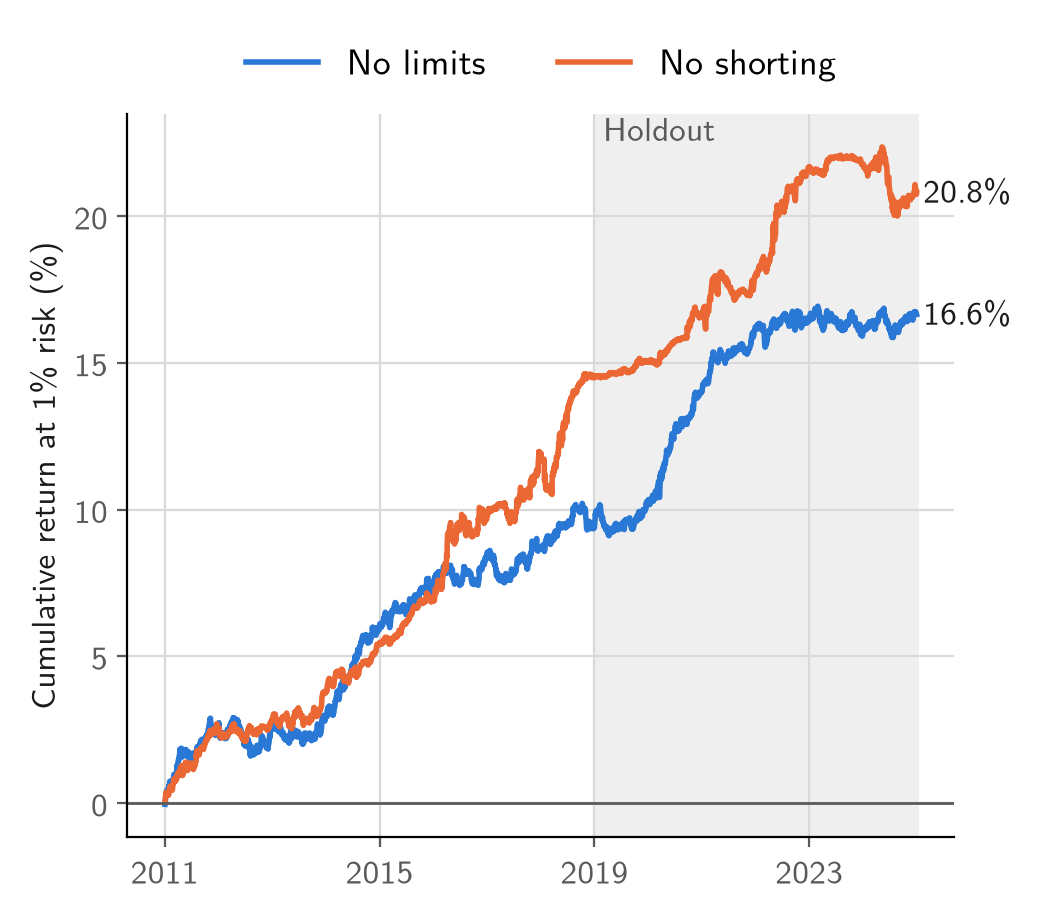
\includegraphics[width=0.55\linewidth]{../slides/figures/pair_daily.png}
\caption{Daily rebalancing: cumulative active return, each period scaled to 1\% risk; shaded years held back.}\label{fig:daily}
\end{figure}

\begin{itemize}
  \item \textbf{Daily holds up.} Long-only earns $+0.51\%$ a year in 2019--2024 (IR 1.05, $t = 2.6$), and the
        no-limits IR (1.21) matches 2011--2018 almost exactly.
  \item \textbf{Monthly does not.} A portfolio that trades once a month reaches most events after their strongest weeks.
  \item \textbf{The optimizer is needed.} Simply selling flagged stocks out of the benchmark earns $+0.05$ to $+0.10\%$
        a year, not significant. Dropping them tilts the portfolio toward large stocks, and that noise swamps the effect.
\end{itemize}

% ======================================================================
\section{How much to trust it}
\takeaway{Encouraging, but small and based on six held-back years.}

\begin{itemize}
  \item \textbf{One honest test.} We refined the design on 2011--2018 in four rounds (Appendix, Table~\ref{tab:versions}),
        then froze it and ran 2019--2024 once.
  \item \textbf{Small.} After bid--ask spreads, daily long-only earns about $+0.3\%$ a year. Its 2019--2024 portfolio is
        larger than before because the model learned that large stocks drift too (Appendix, Table~\ref{tab:size}).
  \item \textbf{Short sample.} An IR's standard error is about $1/\sqrt{\text{years}}$, so six years leaves the true
        long-only IR somewhere between roughly 0.2 and 1.9.
  \item \textbf{Not yet checked.} Thinly traded stocks have stale prices, which can make daily risk look too small.
\end{itemize}

% ======================================================================
\section{Conclusion}
Stocks whose trading dries up keep falling for months: most investors no longer want them, and the hand-off to the few patient buyers is slow. A long-only fund can harvest
this, but only with a volatility-scaled Grinold--Kahn alpha, the optimizer and daily trading. The gain is a few tenths
of a percent a year, so we recommend it as one input to the fund's combined alpha, after a check for stale prices.

% ======================================================================
\appendix
\section{Questions a reader may ask}

\paragraph{Is it just a known effect?} No. Flagged stocks earn less after controlling for size, prior illiquidity,
momentum and reversal (Table~\ref{tab:reg}). The regression is monthly, so it understates the first weeks.
\begin{table}[H]
\centering
\caption{Monthly regressions of next month's specific return, 2008--2018; positive = flagged stocks earn less.
Measured monthly, so it understates the first-weeks effect.}\label{tab:reg}
\small
\begin{tabular}{lr}
\toprule
 & How much less flagged stocks earn, \%/month ($t$) \\
\midrule
Had a liquidity event in the last month & 0.18 (2.5) \\
... also controlling for last month's return & 0.17 (2.4) \\
\bottomrule
\end{tabular}
\end{table}

\paragraph{What did you change, and when?} Each version fixed a problem found in 2011--2018; version 4 was frozen before
2019--2024 was run (Table~\ref{tab:versions}).
\begin{table}[H]
\centering
\caption{The four versions, daily runs, 2011--2018: return \% a year (IR).}\label{tab:versions}
\small
\begin{tabular}{lrr}
\toprule
Daily runs, \%/yr (IR), no costs & No limits & No shorting \\
\midrule
1. Flag that turns over daily & $-0.9$ ($-0.15$) & --- \\
2. Event clock & $-$2.77 ($-$0.49) & $-$0.12 ($-$0.24) \\
3. + no positive alpha, hedge with similar stocks & +3.23 (0.58) & +0.36 (1.48) \\
4. + alpha scaled by volatility & +6.84 (1.17) & +0.19 (1.82) \\
\bottomrule
\end{tabular}
\end{table}

\paragraph{Why is the long-only result bigger in 2019--2024?} Until 2015 the model gave large stocks no alpha, so it could
only sell small stocks with little benchmark weight. Later, large stocks got a negative alpha too (Table~\ref{tab:size}).
\begin{table}[H]
\centering
\caption{Large-stock alpha (first month, per unit of volatility, $\times10{,}000$) and the daily long-only portfolio's
risk and return, by year.}\label{tab:size}
\begin{minipage}{0.5\linewidth}\centering\small
\resizebox{\linewidth}{!}{%
\begin{tabular}{lrrr}
\toprule
 & Large-stock & Long-only & Long-only \\
Year & alpha & risk & return \\
\midrule
2011 & 0.0 & 0.08\% & +0.25\% \\
2012 & 0.0 & 0.06\% & +0.04\% \\
2013 & 0.0 & 0.08\% & +0.10\% \\
2014 & $-$0.1 & 0.07\% & +0.17\% \\
2015 & 0.0 & 0.05\% & +0.16\% \\
2016 & $-$0.8 & 0.15\% & +0.28\% \\
2017 & $-$2.1 & 0.12\% & +0.21\% \\
2018 & $-$3.2 & 0.16\% & +0.29\% \\
\midrule \multicolumn{4}{l}{\textit{Holdout}} \\
2019 & $-$4.9 & 0.16\% & +0.26\% \\
2020 & $-$5.0 & 0.30\% & +0.76\% \\
2021 & $-$7.2 & 0.59\% & +0.63\% \\
2022 & $-$7.1 & 0.68\% & +1.80\% \\
2023 & $-$7.3 & 0.21\% & +0.06\% \\
2024 & $-$7.4 & 0.66\% & $-$0.47\% \\
\bottomrule
\end{tabular}}\end{minipage}
\end{table}

% ======================================================================
\begin{thebibliography}{9}
\bibitem[Amihud(2002)]{amihud2002}
Amihud, Y. (2002). Illiquidity and stock returns: cross-section and time-series effects.
\emph{Journal of Financial Markets}, 5(1), 31--56.

\bibitem[Amihud and Mendelson(1986)]{amihud1986}
Amihud, Y., \& Mendelson, H. (1986). Asset pricing and the bid-ask spread. \emph{Journal of Financial Economics}, 17(2), 223--249.

\bibitem[Bali et~al.(2014)]{bali2014}
Bali, T.~G., Peng, L., Shen, Y., \& Tang, Y. (2014). Liquidity shocks and stock market reactions.
\emph{Review of Financial Studies}, 27(5), 1434--1485.

\bibitem[Clarke et~al.(2002)]{clarke2002}
Clarke, R., de Silva, H., \& Thorley, S. (2002). Portfolio constraints and the fundamental law of
active management. \emph{Financial Analysts Journal}, 58(5), 48--66.

\end{thebibliography}

\end{document}
